\chapter{Psalm 1}

\begin{figure}
  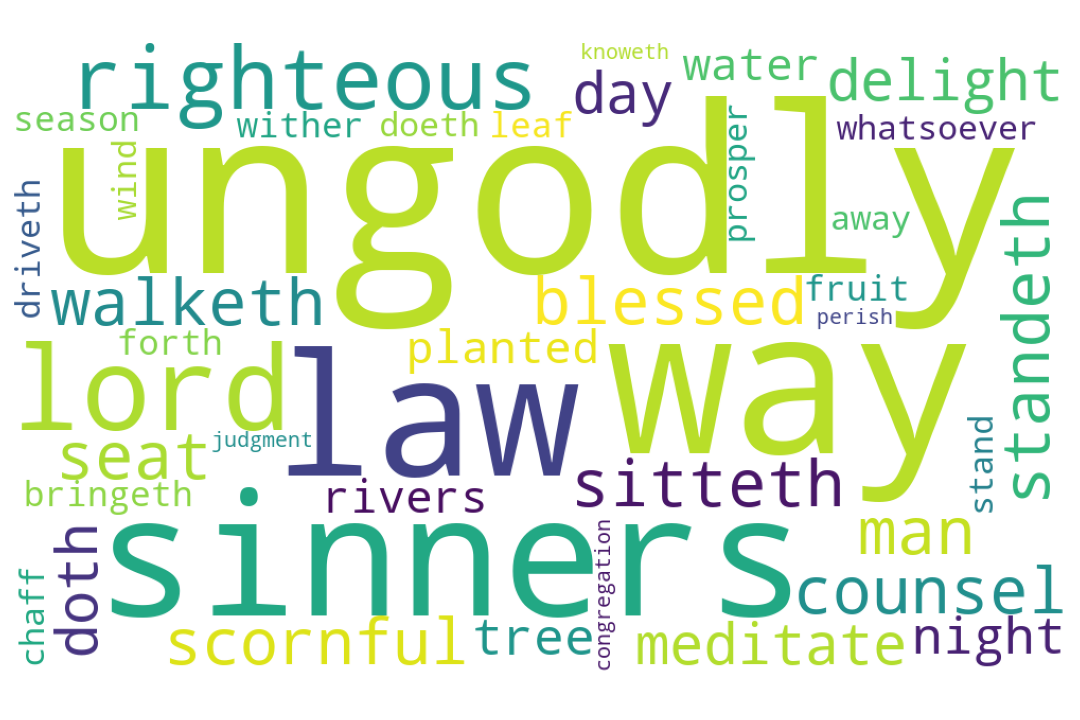
\includegraphics[width=\linewidth]{19OT-Psalms/Psalm1-WordCloud.jpg}
  \caption{Psalm 1 Word Cloud}
  \label{fig:Psalm 1 word Cloud}
\end{figure}


\marginpar{\scriptsize \centering \fcolorbox{bone}{lime}{\textbf{A PSALM OF COMPARISON}}\\ (Psalm 1) 
\begin{compactenum}[I.][8]
    \item A \textbf{Downward Cycle} \index[scripture]{Psalms!Psa 001:01}(Psa 1:1)
    \item A \textbf{Dialobical Counsel} \index[scripture]{Psalms!Psa 001:01}(Psa 1:1)
    \item \textbf{Diligent Consideration} \index[scripture]{Psalms!Psa 001:02}(Psa 1:2)
    \item A \textbf{Different Course} \index[scripture]{Psalms!Psa 001:02}(Psa 1:2)
    \item \textbf{Driven Chaff} \index[scripture]{Psalms!Psa 001:04}(Psa 1:4)
    \item \textbf{Distinguishing Characteristics}  \index[scripture]{Psalms!Psa 001:04}(Psa 1:4)
    \item A \textbf{Delivered Congregation} \index[scripture]{Psalms!Psa 001:05}(Psa 1:5)
    \item A \textbf{Definite Conclusion} \index[scripture]{Psalms!Psa 001:06}(Psa 1:6)
\end{compactenum} }

\marginpar{\scriptsize \centering \fcolorbox{bone}{yellow}{\textbf{THE PSALM 1 MAN}}\\ (Psalm 1) 
\begin{compactenum}[I.][8]
    \item \textbf{Shuns Fools} \index[scripture]{Psalms!Psa 001:01}(Psa 1:1)
    \item Has \textbf{Select Friends} \index[scripture]{Psalms!Psa 001:01}(Psa 1:1)
    \item Eats \textbf{Spiritual Food} \index[scripture]{Psalms!Psa 001:02}(Psa 1:2)
    \item Has \textbf{Special Fellowship} \index[scripture]{Psalms!Psa 001:02}(Psa 1:2)
    \item Exercises \textbf{Simple Faith} (All)
    \item Has his \textbf{Sins Forgiven} (All)
    \item He Can \textbf{Sense Falsehood}
    \item He \textbf{Sees the Future}
    \item Has a \textbf{Spectacular \& Secure Finish} \index[scripture]{Psalms!Psa 001:06}(Psa 1:6)
\end{compactenum}}



\marginpar{\scriptsize \centering \fcolorbox{bone}{black}{\textcolor{white}{\textbf{A COSMIC COMPARISON}}}\\ (Psalm 1) 
\begin{compactenum}[I.]
    \item They have Different \textbf{Objectives}
    \item They have Different \textbf{Orientations}
    \item They have Different \textbf{Obsessions}
    \item They have Different \textbf{Orientations}
    \item They have Different \textbf{Obstacles}
    \item They have Different \textbf{Outcomes}
\end{compactenum}}


\marginpar{\scriptsize \centering \fcolorbox{bone}{blue}{\textcolor{white}{\textbf{ON THE ROAD TO SCORN}}}\\ (Psalm 1) 
\begin{compactenum}[I.]
    \item Not \textbf{Recognizing Blessings}
    \item \textbf{Reviling the Brethren}
    \item Not \textbf{Reading the Book}
    \item \textbf{Revelling in Bitterness}
    \item Not \textbf{Remembering the Burdens}
    \item Not \textbf{Regarding the Body}
    \item Not Carrying the \textbf{Burdens of Believers}
\end{compactenum} }

\marginpar{\scriptsize \centering \fcolorbox{bone}{orange}{\textbf{THE UNGODLY}}\\ (Psalm 1) 

\begin{compactenum}[I.][8]
	\item ungodly \textbf{man} \index[scripture]{Psalms!Psa 001:01}  \index[scripture]{Psalms!Psa 001:04}  \index[scripture]{Psalms!Psa 001:05}  \index[scripture]{Psalms!Psa 003:07}  \index[scripture]{Psalms!Psa 018:04}  \index[scripture]{Proverbs!Pro 16:27} \index[scripture]{Romans!Rom 04:04} (Psa 1:1, 1:4, 1:5, 3:7, 18:4, Pro 16:27, Rom 4:4)
	\item ungoldy \textbf{men} \index[scripture]{2 Samuel!2Sam 22:05} \index[scripture]{2 Chronicles!2Chr 19:02} (2Sam 22:5, 2Chr 19:2, Job 16:11, Job 34:18, Psa 1:6, Psa 73:12, 1Tim 1:9, 1Pet 4:18, 2Pet 2:5, 2Pet 2:6, 2Pet 2:7, Jude 1:4, Jude 1:15)
	  \index[scripture]{Job!Job 16:11}\index[scripture]{Job!Job 34:18} \index[scripture]{Psalms!Psa 001:06} \index[scripture]{Psalms!Psa 073:12}\index[scripture]{1 Timothy!1Tim 01:09} \index[scripture]{1 Peter!1Pet 04:18}\index[scripture]{2 Peter!2Pet 02:05}\index[scripture]{2 Peter!2Pet 02:06}\index[scripture]{2 Peter!2Pet 02:07}\index[scripture]{Jude!Jude 01:15}
	\item ungodly \textbf{nation} \index[scripture]{Psalms!Psa 043:01} (Psa 43:1)
	\item ungodly \textbf{witness} \index[scripture]{Proverbs!Pro 19:28} (Pro 19:28)
	\item ungodly \textbf{deeds} \index[scripture]{Jude!Jude 01:15} (Jude 1:15)
	\item ungodly \textbf{actions} \index[scripture]{Jude!Jude 01:15} (Jude 1:15)
	\item ungodly \textbf{lusts} \index[scripture]{Jude!Jude 01:18} (Jude 1:18)
\end{compactenum}}



\footnote{\textcolor[cmyk]{0.99998,1,0,0}{\hyperlink{TOC}{Return to end of Table of Contents.}}}\footnote{\href{https://www.audioverse.org/english/audiobibles/books/ENGKJV/O/Ps/1}{\textcolor[cmyk]{0.99998,1,0,0}{Psalms Audio}}}\textcolor[cmyk]{0.99998,1,0,0}{Blessed is the man that \fcolorbox{bone}{lime}{walketh} not in the counsel of the \fcolorbox{bone}{lime}{ungodly}, nor \fcolorbox{bone}{lime}{standeth} in the way of sinners, nor \fcolorbox{bone}{lime}{sitteth} in the seat of the scornful.}
[2] \textcolor[cmyk]{0.99998,1,0,0}{But\textcolor{jungle}{$_{29}$} his delight is in the \fcolorbox{bone}{lime}{law of the LORD}; and in his law doth he meditate \fcolorbox{bone}{lime}{day and night}.}
[3] \textcolor[cmyk]{0.99998,1,0,0}{And\textcolor{jungle}{$_{49}$} he shall be like a tree planted by the rivers of water, that bringeth forth his fruit in his season; his leaf also shall not wither; and whatsoever he doeth shall prosper.}\footnote{\textbf{Jeremiah 17:8} -- For he shall be as a tree planted by the waters, and \emph{that} spreadeth out her roots by the river, and shall not see when heat cometh, but her leaf shall be green; and shall not be careful in the year of drought, neither shall cease from yielding fruit.}\footnote{The phrase ``rivers of water'' is found here in Psalm 1:3, Proverbs 21:1, Isaiah 32:2, and Lamentations 3:48. Interestingly, Isaiah 32:2 sets it in a Millennial context.}
[4] \textcolor[cmyk]{0.99998,1,0,0}{The\textcolor{jungle}{$_{82}$} ungodly are not so: but are \fcolorbox{bone}{lime}{like} the \fcolorbox{bone}{lime}{chaff} which the wind driveth away.}\footnote{The word ``chaff'' is found 14 times in 14 verses in scripture, only twice in the New Testament (Mathew 3:12 and Luke 3:17) speaking of the chaff which will be burnt up with unquenchable fire. See: (1) Job 21:18, (2)  Psalm 1:4 (here),  (3) Psalm 35:5, (4)  Isaiah 5:24, (5)  Isaiah 17:13, (6)  Isaiah 29:5, (7) Isaiah 33:11, (8)  Isaiah 41:15, (9) Jeremiah 23:28, (10) Daniel 2:35, (11) Hosea 13:3, (12) Zephaniah 2:2, (13) Matthew 3:12, and (14) Luke 3:17.} 
[5] \textcolor[cmyk]{0.99998,1,0,0}{Therefore\textcolor{jungle}{$_{113}$} the ungodly shall not stand in the judgment, nor sinners in the \fcolorbox{bone}{lime}{congregation} of the righteous.}
[6] \textcolor[cmyk]{0.99998,1,0,0}{For\textcolor{jungle}{$_{114}$} the LORD knoweth the way of the righteous: but the way of the ungodly \fcolorbox{bone}{lime}{shall perish}\textcolor{jungle}{$_{130}$}.}\footnote{\textbf{Psalm 49:12, 17--20} -- Nevertheless man being in honour abideth not: he is like the beasts that perish. [17]  For when he dieth he shall carry nothing away: his glory shall not descend after him.  [18]  Though while he lived he blessed his soul: and men will praise thee, when thou doest well to thyself. [19]  He shall go to the generation of his fathers; they shall never see light.  [20]  Man that is in honour, and understandeth not, is like the beasts that perish.}

